%settings are located in begin_settins.tex and end_settings.tex files
%%%%%%%%%%%%%%%%% do not remove! %%%%%%%%%%%
% mainfile: main.tex
% author Ondrej Platek 2012, settings are without any warranty

%% Verze pro jednostranný tisk:
% Okraje: levý 40mm, pravý 25mm, horní a dolní 25mm
% (ale pozor, LaTeX si sám přidává 1in)
\documentclass[12pt,a4paper]{report}
\setlength\textwidth{145mm}
\setlength\textheight{247mm}
\setlength\oddsidemargin{15mm}
\setlength\evensidemargin{15mm}
\setlength\topmargin{0mm}
\setlength\headsep{0mm}
\setlength\headheight{0mm}
% \openright zařídí, aby následující text začínal na pravé straně knihy
\let\openright=\clearpage

%% Pokud tiskneme oboustranně:
% \documentclass[12pt,a4paper,twoside,openright]{report}
% \setlength\textwidth{145mm}
% \setlength\textheight{247mm}
% \setlength\oddsidemargin{15mm}
% \setlength\evensidemargin{0mm}
% \setlength\topmargin{0mm}
% \setlength\headsep{0mm}
% \setlength\headheight{0mm}
% \let\openright=\cleardoublepage

%% Pokud používáte csLaTeX (doporučeno):
% \usepackage{czech}
%% Pokud nikoliv:
%\usepackage[czech]{babel}
%\usepackage[T1]{fontenc}

%% Použité kódování znaků: obvykle latin2, cp1250 nebo utf8:
% \usepackage[utf8x]{inputenc}

%% Ostatní balíčky
\usepackage{draftwatermark} % really cool draftmark
\SetWatermarkScale{4}
\SetWatermarkLightness{0.7}
%\SetWatermarkText{Draft!}

\usepackage{listings}
\usepackage{graphicx}
\usepackage{amsthm,amsmath,algpseudocode}
\usepackage{cite}

%% Packages needed for Latex-Draw 
%% pretty cool drawing - latex-generating program
\usepackage[usenames,dvipsnames,pdf]{pstricks}
\usepackage{epsfig}
\usepackage{pst-grad} % For gradients
\usepackage{pst-plot} % For axes
\usepackage[chapter]{algorithm}


%% package hyperref, links in PDF,
%% but mainly stores content metadata including content into PDF
\usepackage[unicode]{hyperref}   % HAS TO BE THE LAST PACKAGE 
\hypersetup{pdftitle=Probit regression with Gibbs sampling}
\hypersetup{pdfauthor=Ondřej Plátek}

\title{Probit regression with Gibbs sampling}
\date{1.6.2013}
\author{Ondřej Plátek}

%%% Drobné úpravy stylu

% Tato makra přesvědčují mírně ošklivým trikem LaTeX, aby hlavičky kapitol
% sázel příčetněji a nevynechával nad nimi spoustu místa. Směle ignorujte.
\makeatletter
\def\@makechapterhead#1{
  {\parindent \z@ \raggedright \normalfont
   \Huge\bfseries \thechapter. #1
   \par\nobreak
   \vskip 20\p@
}}
\def\@makeschapterhead#1{
  {\parindent \z@ \raggedright \normalfont
   \Huge\bfseries #1
   \par\nobreak
   \vskip 20\p@
}}
\makeatother

% Toto makro definuje kapitolu, která není očíslovaná, ale je uvedena v obsahu.
\def\chapwithtoc#1{
\chapter*{#1}
\addcontentsline{toc}{chapter}{#1}
}

\def\todo#1{
\emph{\color{red} TODO: #1}
}

\def\todon#1{
  \todo{#1 \\}
}

% references to footnote
% usage: \footnoteremember{myfootnote}{This is my footnote} and then \footnoterecall{myfootnote} 
\newcommand{\footnoteremember}[2]{
    \footnote{#2}
    \newcounter{#1}
    \setcounter{#1}{\value{footnote}}
}
\newcommand{\footnoterecall}[1]{
    \footnotemark[\value{#1}]
}
\begin{document}
\pagestyle{plain}
\setcounter{page}{1}
%\tableofcontents %prida obsah

\theoremstyle{plain}
\newtheorem{thm}{Theorem}[chapter] % reset theorem numbering for each chapter

\theoremstyle{definition}
\newtheorem{defn}[thm]{Definition} % definition numbers are dependent on theorem numbers
\newtheorem{exmp}[thm]{Example} % same for example numbers


\chapter{Gibbs sampling in~probit~regression}
\label{cha:gibbs_sampling_for_probit_regression}


\section{Introduction} 
\label{sec:introduction}
In this short document we would like to introduce {\it Bayesian approach} to {\it probit regression}. In {\it Bayesian theory} we are  trying to derive a distribution for an unknown random variable from already known random variables. 

In our example we would like to know a posterior distribution for the weights $w$ in the~probit regression model. We will derive the posterior distribution from the seen features $x_i$, labels $y_i$ for observations $i\in\{1,\ldots,N\}$ and the prior on weights $w$. We also suppose that each observation from $\{1,\ldots,N\} \cup \{new\}$ are $iid$. 

In fact, we are interested in predictive distribution for the label $y_{new}$ for the unseen features $x_{new}$ based on the knowledge of posterior distribution for~weights. Unfortunately, it is typical that the computation of the posterior and consequently posterior distribution is intractable or even impossible. We will use {\it Gibbs sampling} as a approximation method of drawing samples from the posterior distribution. Obtaining samples from posterior distribution for $Y$ allows us to approximate posterior distribution and later compute predictive distribution for random variable $y_{new}$.


% section introduction (end)

\section{Probit model}
What is a probit model?
\begin{quotation}
    Probit model is a type of regression where the dependent variable can only take two values.
\end{quotation}\cite{wiki_probit}
In our example, the values will be $\{0,1\}$.

\begin{figure}[!hb]
\centering
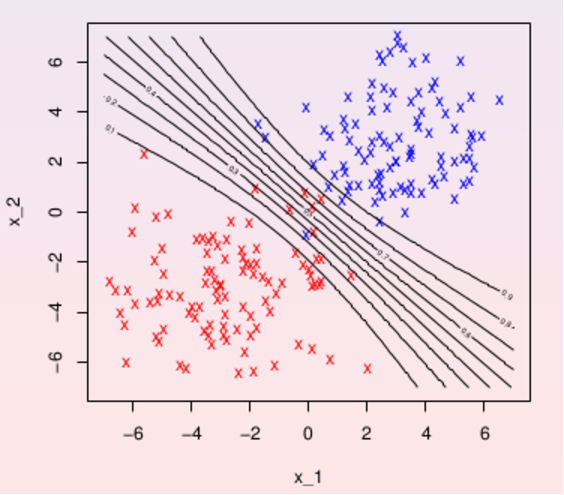
\includegraphics[width=0.8\textwidth]{probit2D}
\caption{Probit regression in dimensions $x_1$ and $x_2$. The separation line is determined by random variable $w$. As expected, the separation line is located with the highest probability between the two differently labeled clusters.}
\label{fig:probit2D}
\end{figure}

\begin{defn}
    In {\bf probit model} we assume that we can describe binary class variable $y_i$ as function of features $x_i$ and parameters $w$:
\begin{align}
    \forall i\in\{1,\ldots,N\} \Pr(y_i=1 \mid x_i) = \Phi(x_i' * w) \\
    \text{or written as vectors: } \Pr(Y=1 \mid X) = \Phi(X' * w)
\end{align}
where $\Phi$ is CDF of standard normal distribution.
\footnote{I will be using $x'$ instead of $x^T$ as mark for vector or matrix transposition.}
\end{defn}

For given features $x_i$ we have the distribution $P(y_i=1 \mid x_i, w)$ which tells us how is probably that the observation falls in class $1$ and not in class $0$ given the features $x_i$ and weights $w$.

Usually, the parameters $w$ are estimated by maximum likelihood. Denote them $w^*$. For new features $x_{new}$ we would give label $y_{new}$ according weights $w*$ and the features $x_{new}$. The problem is that we do not consider any other values for $w*$ even if they are just slightly less probably than $w*$. 

However, in Bayesian theory we put prior on $w$, which means that we consider every possible value for~weights $w$, because $w$ is a random variable. Instead of computing maximum likelihood from already seen data, we compute posterior distribution in equation~\ref{eq:posterior}.
\begin{equation}\label{eq:posterior}
    P(w \mid X, Y) 
\end{equation}
In our case we suppose that $w$ is normally distributed.
\begin{equation}\label{eq:prior_weights}
w \sim \norm(\mu_0, \Sigma_0)
\end{equation}

Usually, the posterior probability~\ref{eq:posterior} is estimated from the likelihood as
\begin{equation}
    P(Y \mid X, w) = \frac{P(w \mid X,Y)}{P(w)},
\end{equation}
where we know $P(w)$ from the~prior~\ref{eq:prior_weights}.
With the posterior probability we may be able to compute predictive distribution 
\begin{equation}
P(y_{new} \mid x_{new},X, Y, w) \overset{iid}{=} P(y_{new} \mid x_{new}, w) = \int_w P(y_{new} \mid x_{new}, w) * P(w) \mathrm{d} w.
\end{equation}

The problem is that we are not able to compute the posterior efficiently. Not even for the latent variable model, which we will introduce in section~\ref{sec:introducing_latent_variale}.

However, we will be able to draw samples from the posterior distribution with Gibbs sampler and latent model.

Let's recapitulate how does probit model look like on example from Figure~\ref{fig:probit2D}.
The weights, $w$, are $d$-dimensional radnom variable. In case of Figure~\ref{fig:probit2D} $d=2$.
The $X$ is $(d*N)$-dimensional matrix, where column $i$ contains $d$-dimensional features $x_i$ of observation $i$.
The $Y$ is $N$-dimensional random vector with output values $y_i \in \{0,1\}$, where $N$ is the number of already seen data ($x_i$ and $y_i$).
The observation $x_i$ on coordinates $x\_1_i,x\_2_i$ is labeled with $1$ if it is blue or $0$ if it is red.

The graphical model in the Figure~\ref{fig:probitGM} illustrates relationships among random variables in probit model. As you can see, each observation $y_i$ of $N$ observation depends on its features $xi$ and also on the weights $w$. We put prior on weights $w$ as a distribution with parameters $\mu_0$ and $\Sigma_0$. The graphical also models depicts that we observe $N$ times the features $x_i$ and the class label $y_i$ for different $iid$ observations $i$.

\begin{figure}[!hb]
\centering
% Generated with LaTeXDraw 2.0.8
% Sat Jun 01 00:47:45 CEST 2013
% \usepackage[usenames,dvipsnames]{pstricks}
% \usepackage{epsfig}
% \usepackage{pst-grad} % For gradients
% \usepackage{pst-plot} % For axes
\scalebox{1} % Change this value to rescale the drawing.
{
\begin{pspicture}(0,-2.59)(6.041875,2.59)
\psframe[linewidth=0.04,dimen=outer](2.76,2.59)(0.0,-2.59)
\pscircle[linewidth=0.04,dimen=outer](1.2942857,-0.68918365){0.4542857}
\pscircle[linewidth=0.04,dimen=outer](1.31,-0.7){0.53}
\psline[linewidth=0.055999998cm,tbarsize=0.07055555cm 5.0,arrowsize=0.05291667cm 2.0,arrowlength=1.4,arrowinset=0.4]{|*->}(1.34,1.49)(1.34,-0.21)
\pscircle[linewidth=0.04,dimen=outer](4.4142857,-0.7291837){0.4542857}
\psline[linewidth=0.055999998cm,tbarsize=0.07055555cm 5.0,arrowsize=0.05291667cm 2.0,arrowlength=1.4,arrowinset=0.4]{|->}(4.38,1.59)(4.38,-0.27)
\psline[linewidth=0.055999998cm,arrowsize=0.05291667cm 2.0,arrowlength=1.4,arrowinset=0.4]{->}(3.98,-0.73)(1.722,-0.73)
\usefont{T1}{ptm}{m}{n}
\rput(1.9514062,1.675){$x_i$}
\usefont{T1}{ptm}{m}{n}
\rput(4.5914063,1.735){$\mu_0, \Sigma_0$}
\usefont{T1}{ptm}{m}{n}
\rput(5.1714063,-0.185){$w$}
\usefont{T1}{ptm}{m}{n}
\rput(2.2514062,-2.045){$N$}
\usefont{T1}{ptm}{m}{n}
\rput(0.38140625,-0.305){$y_i$}
\end{pspicture} 
}


\caption{Graphical model for Probit}
\label{fig:probitGM}
\end{figure}

\section{Introducing latent variable $\Yh$ }
\label{sec:introducing_latent_variale}
In fact, the model with latent variable is just technical trick. Later, in section~\ref{sec:sampling_from_marginal_distribution_in_probit_example} we will find out that the Gibbs sampler needs to draw samples from marginal distributions for each variable of joint distribution we want to sample from. In the probit model we do not know how to compute the marginal distributions.

However we are able to draw samples from marginal distributions of the model with latent variable, which we will introduce in this section. Furthermore, we can easily convert the latent model to probit model. So if we can draw samples from latent model we can draw samples from the probit model, which is our goal.

Let us introduce the latent model and remind priors on distribution for the random variables.
\begin{equation}\label{eq:lat}
    \Yh = X' * w + \varepsilon, 
\end{equation}
where we suppose that:
\begin{itemize}
    \item weights $w$ are distributed according the~equation~\ref{eq:prior_weights} 
    \item noisy labeling without loss of generality\footnote{Without loss of generality we can assume $\norm(0,1)$ instead of $\varepsilon \sim \norm(0, S)$. 
        If we needed to estimate weights $w$ for $\norm(0, S)$ introduced in the~graphical model we will estimate weights $w^h$ for $\norm(0,1)$ and set $w = S*w^h$}
        \begin{equation}\label{eq:noise}
        \varepsilon \sim \norm(0, 1).
        \end{equation}
    \item $X$ is the matrix of features, \\
\end{itemize}

Note that we can draw samples from the probit model if we can draw samples from $\overset{\sim}{y_{i}}$ by applying following rule.
\begin{equation}\label{eq:model_equivalence}
    y_i = 
     \begin{cases} 
         1 & \text{if }\yh > 0 \ \text{ i.e. } - \varepsilon < x_i' * w, \\
         0 &\text{otherwise.} 
     \end{cases}
\end{equation}
Let us prove that equation~\ref{eq:model_equivalence} determines the probit model.
\begin{align}
    P(y_i=1 \mid x_i) &= P(\yh > 0 ) = P(x_i' * w + \varepsilon > 0) \\
                      &= P(\varepsilon > - x_i' * w) \\
                      &= P(\varepsilon > - x_i' * w) \\
    \text{by symmetry of normal distribution} \\
                      &= P(\varepsilon < x_i' * w) \\
                      &= \Phi(x_i' * w)
\end{align}



\section{Sampling from model with latent variable} 
\label{sec:sampling_from_model_with_latent_variable}
Let us shortly recapitulate facts. We know that feature vectors $x_i$ are represented compactly in matrix $X$. There is label $y_i \in \{0,1\}$ for each of vector $x_i$. Labels are compactly represented as $Y$. We assume that $\varepsilon$, $w$ random variables are normally distributed and we do not know parameters for $w$ yet.

Firstly, we will introduce the Gibbs sampling algorithm. Secondly, we will derive the marginal distributions needed by Gibbs sampling. Finally, at the end we will summarize what can we deduce from the samples about distributions which interest us.

\subsection*{Gibbs sampler}
\label{sub:gibbs_sampler}
\begin{quote}
The point of Gibbs sampling is that given a multivariate distribution it is simpler to sample from a conditional distribution than to marginalize by integrating over a joint distribution. \cite{wiki_gibbs}
\end{quote}
We will describe Gibbs sampling algorithm and claim some facts. We will not proved the properties. See the references into literature for details. However, we will derive the in detail the marginal distributions which are necessary for running Gibbs sampler.

\subsubsection*{How does Gibbs sampling work?}
Suppose we want to sample from $Z = \{z_1, z_2, \ldots, z_l\}$ with distribution $P(z_1, z_2, \ldots, z_l)$. Let us denote the $k^{th}$ sample from $Z$ by $Z^k = \{z_1^k, z_2^k, \ldots, z_l^k\}$. The Gibbs algorithm will sample $Z^k$ according pseudo code below. For large enough $k$ the distribution, from which the samples $Z^k, Z^{k+1}, \ldots $ are drawn, will converge to distribution $P(z_1, z_2, \ldots, z_l)$. 


\begin{algorithm}
\caption{Gibbs algorithm} \label{gibbs_pseudo}
\begin{algorithmic}
\State k=0
\State $Z^k$ = InitValues()
\Comment{Somehow initialize the vector $:Z^k$}
\While{Samples did not converge}
    \State  k++
    \Comment{We are sampling $k^{th}$ sample}
    \For{ $j \in \{1,\ldots, l\}$ }
        \State $z_j^k \sim P(z_j^k  \mid z_1^k,z_2^k, \ldots, z_{j-1}^k, z_{j+1}^{k-1}, \ldots, z_{n}^{k-1})$
        \Comment{Sampling $z_j^k$}
    \EndFor
\EndWhile
\end{algorithmic}
\end{algorithm}

In following section we will focus on how to sample from the marginal distributions. Now let us deal with the unspecified parts in the algorithm description apart from sampling from marginal distributions.

Firstly, initializing the values is not very problematic. Gibbs sampling is guaranteed to converge for any values. On the other hand, reasonable settings like mean or mode, if we know them,  gives faster convergence than outliers. \cite{gibbs_intro}

Secondly, the stopping condition for Gibbs algorithm is much harder problem. There are several heuristics like autocorrelation metrics or measuring discrepancy between samples and the desired distribution which are trying to detect whether the samples have converged to stable distribution. It can be shown that for Gibbs sampler the stable distribution is in fact the desired $P(Z)$ distribution. \cite{explaining_gibbs}

% subsection introducing_latent_variale (end)

\subsection{Sampling from marginal distribution in Probit example} 
\label{sec:sampling_from_marginal_distribution_in_probit_example}
At the beginning we will give again short and dense overview of facts in few equations. Later we will compute marginals for joint probability $P(w, \Yh \mid X, Y)$. The marginals which we need to compute are 
\begin{itemize}
    \item $P(\Yh \mid w, X, Y)$.
    \item $P(w \mid X, \Yh, Y)$.
\end{itemize}

We assume probit model for $Y$ binary random variable $ Y = \Phi(X' * w)$ where $w$ is distributed as described in equation~\ref{eq:prior_weights}.
Further, without loss of generality we can assume that the latent model is normally distributed with covariance 1 as described below in equation~\ref{eq:cov1}.
\footnote{We can compensate different variance from 1 by setting different variance in prior on weights~$w$ \todo{add equation}}
\begin{equation}\label{eq:cov1}
    \yh \mid x_i, w \overset{ind}{\sim} \norm(x_i' * w, 1)
\end{equation}

From transformation between labels $y_i$ and latent random variable $\yh$ in equation~\ref{eq:model_equivalence} we derive distribution described in terms of truncated normal.
\footnote{More about truncated normal distribution on \href{http://en.wikipedia.org/wiki/Truncated_normal_distribution}{Wikipedia}}
\begin{equation}
    y_i \mid \yh, x_i, w \sim y_i \mid \yh \overset{ind}{\sim} 1(\yh \ge 0)
\end{equation}

\begin{thm}
    All full marginal distributions with variables $w$, $\Yh$ for~joint probability $P(w, \Yh \mid X, Y)$ are distributed according
\begin{enumerate}
\item
    \begin{equation}\label{eq:margin_w}
    w \mid \Yh, X, Y \sim \norm(\hat{w},\hat{\Sigma})
    \end{equation} 
    where 
    $ \hat{\Sigma} = {(\Sigma_0^{-1} + X' * X)}^{-1} $ 
    and
    $ \hat{w} = \hat{\Sigma} ( \Sigma_0^{-1}*\mu_0 + X' * \overset{\sim}{y} ) $

\item 
    \begin{equation}\label{eq:margin_ytilda}
        \Yh \mid w, X, Y \text{ has density } \\
        \prod_{i=1}^{N} Z * \norm(x_i, 1) * {(1(\yh \ge 0))}^{y_i} * {(1(\yh < 0))}^{1-y_i}
    \end{equation} 
    where $Z$ is normalizing constant.
\end{enumerate}
\end{thm}

\begin{proof}
Let us prove the marginal distribution from equation~\ref{eq:margin_w} 
We start with
\begin{equation}
    P(w \mid \Yh, X, Y) 
\end{equation}
and by applying the Bayes rule and omitting the denominator we get
\begin{equation}
    \propto   P(\Yh, Y \mid X, w) * P(w).
\end{equation}
We further expand the first probability by chain rule
\begin{equation}
    \propto   P(\Yh \mid X, w) * P(Y \mid \Yh,  X, w) * P(w).
\end{equation}
The middle term will disappear, because it is our deterministic way how to convert hidden model to probit model.
\begin{equation}
    \propto   P(w) * P(\Yh \mid X, w)
\end{equation}
We can write down the prior on weights. The observations are $iid$ distributed, so we can use the product of their distributions. Further, we assume without loss of generality that \todo{  the latent model has variance 1 for each observation}.
\begin{align}
    &= \norm(\mu_0, \Sigma_0) * \prod_{i=1}^N \norm(\yh \mid x_i' * w, 1) \\
    &\propto \norm(\mu_0, \Sigma_0) * \norm(\Yh \mid X' * w, \unity_N) \label{eq:w_marg_vect}\\
    &= \norm \left(w  \mid  (\color{orange}\Sigma_0^{-1} + XX')^{-1}(\Sigma_0^{-1}\mu_0 + X\Yh\color{black}), (\Sigma_0^{-1} + XX')^{-1}\right) \label{eq:w_marg_final} \\
    &= \norm \left(w  \mid  \color{orange}\hat{\mu}\color{black}, \hat{\Sigma}\right)  \text{ We denote the new mean and covariance $\hat{\mu}$ and $\hat{\Sigma}$}
\end{align}

Let us explain how we derive $\hat{\mu}$ and $\hat{\Sigma}$ from equation~\ref{eq:w_marg_vect}.
\begin{align}
& \norm(w \mid \mu_0, \Sigma_0) * \norm(\Yh \mid X'w, \unity_N) = \\
&= \frac{1}{\sqrt{(2\pi)^N|\Sigma_0|}}\exp({-\frac{1}{2}(w-\mu_0)'\Sigma_0^{-1}(w-\mu_0)}) * 
    \notag\\ &\mspace{50mu} 
    * \frac{1}{\sqrt{(2\pi)^N|\unity_N|}}\exp({-\frac{1}{2}(\Yh-X'w)'\unity_N^{-1}(\Yh-X'w)}) = \\
&= \frac{1}{(2\pi)^N \sqrt{|\Sigma_0|}}\exp({-\frac{1}{2}[((w-\mu_0)'\Sigma_0^{-1}(w-\mu_0) +  (\Yh-X'w)'(\Yh-X'w)]}) \\
&= c* \exp({-\frac{1}{2}[(w-\mu_0)'\Sigma_0^{-1}(w-\mu_0) +  (\Yh-X'w)'(\Yh-X'w)]}) \\
&= c* \exp({-\frac{1}{2}[w'\Sigma_0^{-1} w - 2w'\Sigma_0^{-1}\mu_0 + \color{blue}\mu_0'\Sigma_0^{-1}\mu_0 + \Yh'\Yh \color{black}-2\Yh'X'w  + w'XX'w]}) \\
&= c* \color{blue} c' \color{black} * \exp({-\frac{1}{2}[w'\Sigma_0^{-1} w - 2w'(\Sigma_0^{-1}\mu_0  + 'X\Yh)  + w'XX'w]}) \\
&= c* \color{blue} c' \color{black} * \exp({-\frac{1}{2}[w'(\Sigma_0^{-1} + XX') w - 2w'(\Sigma_0^{-1}\mu_0  + X\Yh)]}) \\
&= c* \color{blue} c' *\color{violet} c'' \color{black} * \exp (-\frac{1}{2}[w'(\Sigma_0^{-1} + XX') w 
    \notag\\ &\mspace{50mu} 
    - 2w'(\color{orange}\Sigma_0^{-1}\mu_0  + X\Yh)(\Sigma_0^{-1} + XX')^{-1}\color{black} * (\Sigma_0^{-1} + XX')
    \notag\\ &\mspace{50mu} 
\color{violet}(\Sigma_0^{-1} + XX')^{-1}(\Sigma_0^{-1}\mu_0 + X\Yh)'(\Sigma_0^{-1} + XX')(\Sigma_0^{-1} + XX')^{-1}(\Sigma_0^{-1}\mu_0 + X\Yh)\color{black}  ]) \\
&= c* \color{blue} c' *\color{violet} c'' \color{black} * \exp \left(-\frac{1}{2}(w - \color{orange}\hat{\mu}\color{black})' (\Sigma_0^{-1} + XX')(w - \color{orange}\hat{\mu}\color{black}) \right)
\end{align}
\end{proof}

\begin{proof}
Let us prove the second marginal distribution from equation~\ref{eq:margin_ytilda} 
\begin{equation}
P(\Yh \mid X, Y, w) \propto
\end{equation}
We continue by using Bayes rule in form $ P(A \mid C, B) = \frac{P( B \mid A, C) * P(A|C)}{P(B)}$ 
\begin{equation}
    \propto P(\Yh \mid X, w) * P(Y \mid X,\Yh, w)
\end{equation}
Now we substitute the conditional probabilities by: 
\begin{equation}\label{eq:exp_trick}
    P(\Yh \mid X, w) = \prod_{i=1}^{N}\norm(\yh \mid w^T*x_i, 1) \text{ and } 
    P(Y \mid X,\Yh, w) = \prod_{i=1}^{N}{(1_{(\yh \ge 0)})}^{y_i} * {(1_{(\yh < 0)})}^{1-y_i}.
\end{equation}
Note the nice technical trick in equation~\ref{eq:exp_trick}. Instead of writing the {\it if statement} like in equation~\ref{eq:model_equivalence} we wrote ${(1_{(\yh \ge 0)})}^{y_i} * {(1_{(\yh < 0)})}^{1-y_i}$. The first multiplier is 1 if $y_i =0 $ and the second one is 1 if $y_i=1$. Consequently, It leads us to equation for density function point $\Yhs$.
\begin{equation}
P(\Yh = \Yhs \mid X, Y, w)
    \propto \prod_{i=1}^{N}\norm(\yhs \mid w^T*x_i, 1) * 
    \prod_{i=1}^{N}{(1_{(\yhs \ge 0)})}^{y_i} * {(1_{(\yhs < 0)})}^{1-y_i}
\end{equation}

It means that distributions $ P(\yh \mid  x_i, y_i, w) $ are conditionally independent with truncated normal distribution.
\end{proof}

    % slide 6 NPFL108-slidesLexture6-7-SamplingMethods.pdf

\section{Summary} 
\label{sec:summary}
At the beginning we wanted to compute the posterior probability~\ref{eq:posterior}. We come up with the idea of Gibbs sampling which has the advantage that it needs only all full marginal distributions to sample from the joint distribution or some of the marginals. The marginal distributions are generally in more simpler form. Further,sampling is usually much more feasible approximation than other alternatives. 

In our example, we used a latent variable model, because we were not able to derive the distributions for the marginals in probit model. We computed the marginals for latent variable model and then we used the Gibbs sampling method to draw sample from the posterior distribution.

Usually, we are not satisfied with the posterior distribution and we want to compute the predictive distribution. From the samples we estimate the parameters of the posterior distribution and then use it to compute predictive distribution.
\todo{PREDICTIVE Distribution}


% section summary (end)

% section sampling_from_marginal_distribution_in_probit_example (end)


\section*{References}
\begin{itemize}
    \item Git repository for this article \url{https://github.com/bayesian-inference/notes}
    \item This article was written for the \href{https://sites.google.com/site/filipjurcicek/teaching/bayesian-inference}{Bayesian Inference course at MFF UK}
    \item This article is based on Sara's Wade talk for the Bayesian Inference course recorded on \href{http://youtu.be/rsUt9uV6j70?t=12m18s}{Youtube}
    \item The Figure~\ref{fig:probit2D} is taken from \href{https://sites.google.com/site/filipjurcicek/teaching/bayesian-inference/NPFL108-slidesLecture3.pdf?attredirects=0}{slides of Jose Miguel Hernandez-Lobato} given for Bayesian Inference course
\end{itemize}
\bibliographystyle{apalike}
\bibliography{refer}


% chapter gibbs_sampling_for_probit_regression (end)
\end{document}
